%
% instructions for "compiling":
%   latex main (first pass, also generates .aux file for bibtex)
%   bibtex main (generates .bbl file with bibliography)
%   latex main (second pass, incorporates bibliography)
%   latex main (do this if you still get messages about labels
%      having changed or missing references)
% to generate/view/print postscript:
%   dvips -o main.ps main 
%   gv main.ps (to view)
%   lpr main.ps (to print, or print from "gv")
% to generate/view/print PDF:
%   dvips -Pcmz -Ppdf -j0 -G0 -o main.ps main
%   ps2pdf main.ps main.pdf
%   acroread main.pdf (to view/print)
%   
\documentclass[11pt]{report}

% miscellaneous packages
% FIX THIS -- can add to or change, but these are useful
\usepackage{amsmath}
\usepackage{graphicx}
\usepackage{amssymb}
\usepackage{epstopdf}
\DeclareGraphicsRule{.tif}{png}{.png}{`convert #1 `dirname #1`/`basename #1 .tif`.png}

\usepackage{moreverb}
\usepackage{url}

% double spacing
\usepackage{setspace}
\doublespacing

% hyphenation
\usepackage[english]{babel}
\selectlanguage{english}

% allow more figures on a page
\setcounter{topnumber}{10}
\setcounter{bottomnumber}{10}
\setcounter{totalnumber}{10}
\setcounter{dbltopnumber}{10}
\def\topfraction{1.0}
\def\bottomfraction{1.0}
\def\textfraction{0.0}
\def\dbltopfraction{1.0}

\usepackage[retainorgcmds]{IEEEtrantools}

% margins
%\usepackage[letterpaper,top=2.0in,bottom=1.5in,left=1.5in,right=1.0in]
%	{geometry}
\usepackage[top=2.0in,bottom=1.5in,left=1.5in,right=1.0in]{geometry}

% set up to put page numbers in header
\usepackage{fancyhdr}
\pagestyle{fancy}
\lhead{}
\chead{}
\rhead{\rm\thepage}
\lfoot{}
\cfoot{}
\rfoot{}
\renewcommand{\headrulewidth}{0pt}
\renewcommand{\footrulewidth}{0pt}

% author, title, and date
% FIX THIS
\newcommand{\theAuthor}{Ryan Tanner}
% FIX THIS -- but be sure to leave in \par if title might exceed
%   one line -- otherwise space between lines will be wrong
\newcommand{\theTitle}{Creating a Semantic Graph from Wikipedia\par}
% FIX THIS
\newcommand{\theDate}{April 1, 2012}

\usepackage[caption=false]{subfig}

\usepackage{listings}
 
% "define" Scala
\lstdefinelanguage{scala}{
  morekeywords={abstract,case,catch,class,def,%
    do,else,extends,false,final,finally,%
    for,if,implicit,import,match,mixin,%
    new,null,object,override,package,%
    private,protected,requires,return,sealed,%
    super,this,throw,trait,true,try,%
    type,val,var,while,with,yield},
  otherkeywords={=>,<-,<\%,<:,>:,\#,@},
  sensitive=true,
  morecomment=[l]{//},
  morecomment=[n]{/*}{*/},
  morestring=[b]",
  morestring=[b]',
  morestring=[b]"""
}

\usepackage{color}
\definecolor{dkgreen}{rgb}{0,0.6,0}
\definecolor{gray}{rgb}{0.5,0.5,0.5}
\definecolor{mauve}{rgb}{0.58,0,0.82}
 
% Default settings for code listings
\lstdefinestyle{mystyle}{frame=tb,
  aboveskip=3mm,
  belowskip=3mm,
  showstringspaces=false,
  columns=flexible,
  basicstyle={\small\ttfamily},
  numbers=left,
  numberstyle=\tiny\color{gray},
  keywordstyle=\color{blue},
  commentstyle=\color{dkgreen},
  stringstyle=\color{mauve},
  frame=single,
  breaklines=true,
  breakatwhitespace=true
  tabsize=3
}

\lstdefinestyle{scalastyle}{language=scala, style=mystyle}

\lstdefinestyle{xmlstyle}{langauge=xml, style=mystyle}


% FIX THIS -- can put additional macro definitions here

%----------------------------------------------------------------------

\begin{document}

\pagenumbering{gobble}

%
% spacing could probably be improved
%

\begin{center}

\bigskip

\begin{Large}
\textbf{\theTitle}
\end{Large}

\bigskip

\begin{large}
\theAuthor
\end{large}

\bigskip
\bigskip

\textbf{Abstract}

\end{center}

\noindent

With the continued need to organize and automate the use of data, solutions are needed to transform unstructred text into structred information.  By treating dependency grammar functions as programming language functions, this process produces ``property maps'' which connect entities (people, places, events) with snippets of information.  These maps are used to construct a semantic graph.  By inputting Wikipedia, a large graph of information is produced representing a section of history.  The resulting graph allows a user to quickly browse a topic and view the interconnections between entities across history.


\clearpage
%
% spacing could probably be improved
%
\begin{center}

\bigskip

\begin{Large}
\textbf{Acknowledgments}
\end{Large}

\bigskip

\end{center}

%FIX THIS --- thank your advisor, etc., here.
I would like to thank Dr.~Lewis for being my thesis advisor and agreeing to oversee this project despite my complete lack of experience in any area I have covered here.  Our discussions on Scala over the past year have also been excellently entertaining.

In addition, I would like to thank the members of my thesis committee, Dr.~Myers, Dr.~Eggen and Dr.~Lewis.

I would like to recognize Dr.~Hicks, my academic advisor.

I would also like to thank Dr.~Massingill for her technical advice and Neal Pape of Trinity University's ITS department for his assistance in procuring a MySQL database and access to the Dias research machines.  Furthermore I would like to thank Dr.~Zhang for permitting the use of those machines.

For their open-source efforts I would like to recognize the Stanford Natural Language Processing Group and their excellent NLP library.  I would like to thank the Wikimedia Foundation for their caretaking of Wikipedia and thoughtfulness in providing such a wonderful resource in a research-friendly license.


\clearpage
\begin{center}

\vfill

\textbf{\theTitle} %\\

\theAuthor \\

\vspace*{\baselineskip}

A departmental thesis submitted to the \\
Department of Computer Science at Trinity University \\
in partial fulfillment of the requirements for Graduation.\\
% with departmental honors. 

\vspace*{\baselineskip}

\theDate

\vfill

$\overline{\mbox{\rule{0in}{0.16in}Thesis Advisor~~~~~~~~~~~~~~~~~~~~~~~~~~}}$ 
\hfill
$\overline{\mbox{\rule{0in}{0.16in}Department Chair~~~~~~~~~~~~~~~~~~~~~~~~}}$ 

\vspace{1.0in}

$\overline{\mbox{\rule{0in}{0.16in}
~~~~~~~~Associate Vice President~~~~~~~~
}}$ \\
for \\
Academic Affairs

\vfill

\hfill
\hfill
\hfill

\begin{tiny}
%This work is licensed under the Creative Commons Attribution-NonCommercial-NoDerivs License.  To view a copy of this license, visit <http://creativecommons.org/licenses/by-nc-nd/2.0/> or send a letter to Creative Commons, 559 Nathan Abbott Way, Stanford, California 94305, USA.
This work is licensed under the Creative Commons Attribution-NonCommercial-NoDerivs License.  To view a copy of this license, visit \textless http://creativecommons.org/licenses/by-nc-nd/2.0/\textgreater or send a letter to Creative Commons, 559 Nathan Abbott Way, Stanford, California 94305, USA.
\end{tiny}


\end{center}


\clearpage
%
% spacing could probably be improved
%

\begin{center}

\vfill

\begin{Huge}
\textbf{\theTitle}
\end{Huge}

\bigskip \bigskip \bigskip

\begin{huge}
\theAuthor
\end{huge}

\vfill

\end{center}


\tableofcontents
\listoffigures

\clearpage
\pagenumbering{arabic}

% FIX THIS -- one file per chapter is good but not required
\chapter{Introduction}

This thesis is an attempt to construct a semantic graph of entities (people, places, and things) from a large data source in an efficient and effective manner.  Accomplishing this goal requires a solution which is broken down into several components: grammatical parsing, semantic interpretation, and graph construction.  Together these three disparate parts produce a semantic graph which can be quickly traversed to extract relationships and connections between its constituent entities.

In real-world terms, this is an attempt to visualize Wikipedia in a fashion which allows one to quickly find and examine connections between the people, places and things described in Wikipedia.

Other attempts have been made to produce similar visualizations based on the link structure of Wikipedia---the graph formed by user-produced hyperlinks between Wikipedia articles.  These solutions, while effective, do little to add context or reasoning behind their connections.  The WikiViz project \cite{wikiviz} is one such attempt.

While interesting, such an approach ignores the rich quantities of information included in Wikipedia.  Over four million articles in the English language edition alone---26 million across all languages---and without a solution based upon natural language processing the information contained as written word goes unused.  

This solution uses natural language processing to produce context and justification for the connections in the resulting graph.  This forms a central aspect of this thesis: the treatment of dependency functions as first-class functions.  Essentially, the ``language'' of dependency grammars is treated as a functional language, borrowing several aspects from programming language theory.  
 
\chapter{Problem Statement}

This thesis is an attempt to tackle the problem of extracting facts and connections from written text.  Massive quantities of text are produced daily and methods for quickly getting relevant information out of that text are needed.  Furthermore, within these large bodies of text lie the semantics underpinning human knowledge. Extracting these semantics is as of yet a largely unsolved problem though many attempts have been made. 

The internet consists largely of unstructured information.  That is, information written in ordinary language to be read by humans.  Structured information is organized in a fashion computers can trivially utilize such a database of election results or weather information.  Data of this nature has some form of a schema attached which aids computers in deciphering and putting to use an information source.  While we can read and infer a great deal from unstructured information, computers can do much less.

The most obvious solution to this problem is that presented by Google in the form of its search engine.  This uses what structure is available (the hyperlink nature of the internet) and does its best to categorize and index available information.  While very effective---none of us can imagine a day without Google anymore---this approach does not fundamentally try to extract information but merely ranks and scores it.  

Tim Berners-Lee, inventor of the world wide web, refers to the current state of the internet as a ``web of documents'' and hopes to see the rise of the ``web of data''---documents annotated with semantic metadata.  His goal is a system in which any type of data can be organized and hyperlinked creating a global graph spanning numerous disparate sources and categories \cite{RN25892292820090101}.

The field of information extraction revolves around this problem.  Many approaches focus on a small subset of information such as extracting political news from newswire reports.  Others have a generic approach and some of these techniques are used in this project including named entity recognition and coreference resolution.  

\section{Extracting properties defined in a massively large body of text}

For a semantic graph of this nature to be constructed methods are needed which can extract the necessary properties from large bodies of text.  This is the core problem in creating a semantic graph of a source like Wikipedia.  

Much of the difficulty comes from determining what such properties should convey.  If one makes them too generic the graph will be of little use as connections will lack the context needed to understand why such a connection makes sense.  If the properties are too specific the construction of the graph becomes hopelessly complex.  A balance must be struck which allows for an algorithmic approach while still providing the necessary context.

Because a single fact can be conveyed in a virtually countless number of ways in the English language, any solution must be able to cope with extracting a fact in many ways.  The twin fields of natural language processing and information extraction are heavily involved in this but this problem still poses a significant challenge.  My use of dependency grammars is an attempt to work around this problem by first transforming sentences into a consistent structure before extracting any properties.  In this way different sentences become the same when viewed as their representative dependency trees.

\section{Motivation}

This project can be divided into two broad sections and their motivations will be dealt with separately.

First, the language processing component. The use of dependency grammar over the more widely-used constituent grammar was motivated by a desire to test the possibility of applying functional (programming) language concepts to natural language.  More colloquially, I wanted to scratch an intellectual itch.  Treating grammatical functions as computation functions and modeling them as such appealed to me as an elegant proposition.  I freely admit that I had no basis for this approach.  Building this project seemed the best way to test my hypothesis.

The second motivation was the desire to construct a semantic graph which could visualize a topic.  Such a graph would be navigable by the user such that one could find connections between people, places and events related to a topic and see their connections and the reasons justifying those connections.  

\chapter{Other Approaches}

\section{Semantic Web}

Large amounts of data have been quantified and indexed in efforts to construct the ``semantic web.''  ``Data is seamlessly woven together from disparate sources, and new knowledge is derived from the confluence.  This is the vision of the semantic web,'' \cite{semweb} and this vision has been largely realized over the past half-decade.  These efforts center around structuring data in a meaningful and predictable fashion such as Google's map API which provides such a structure for geographical information.  Other sources include LinkedIn's API which gives users access to social graph information, a related field, and Freebase, a semantic database providing a graph of data on a wide range of topics such as art, sports and government.

Some of these sources are community driven, such as Freebase, allowing a wide range of users to collaborate in producing a structured source of data.  Others, like LinkedIn, are powered by social networks.  This notion allows actions already performed by users for other tasks (such as connecting with friends or searching for jobs in the case of LinkedIn) to become the data backing a social graph, quantifying the relationships and connections between users.  A third category of data within the semantic web is statistics and tabular information.  Google Fusion Tables is a product aimed at annotating and organizing such information.

Fusion Tables helps developers organize, visualize and publish data from multiple sources.  A pioneering user of this service is The Texas Tribune, a media organization focusing on public policy in the state of Texas \cite{textrib}.  One such example is their use of Fusion Tables to visualize the set of journalists killed in Mexico \cite{texjour} \cite{texjour1}.  Importantly, Fusion Tables allows users to rapidly combine disparate datasets.

These and other efforts to build the semantic web provide a far simpler means of accessing and utilizing data but at the up-front cost of time and effort in building these datasets.  Many are compiled by hand or consist of data that is naturally amenable to such quantification such as LinkedIn's social graph.  Others are composed of sets of statistics released by governments and research organizations in computer-friendly formats.  While appropriate for some data sources, these techniques are difficult to automate and must be explicitly tailored for their specific source.

A principle challenge of this approach is the problem of free text---text which is completely unstructured.  The automatic or semi-automatic annotation of such text is still not a reliably practical.

\section{Other NLP Work with Wikipedia}

While a great deal of work regarding natural language processing, information retrieval and Wikipedia has been done, I have not found any research directed towards the same end result as my own.  The following is a sample of work done in related arenas:

Ruiz-Casado et al \cite{Ruiz-casado05automaticassignment} used Wikipedia to automatically assign articles to concepts in a lexical or semantic network in order to extend the synsets used by Wordnet.  A synset is a set of synonyms \cite{nlpbook}.  Notably their work uses the Simple English version of Wikipedia in order to simplify their solution.  They found that their approach was significantly more accurate than the previous state-of-the-art for word sense disambiguation.

M\"ulcer and Gurevych \cite{Muller:2008:UWW:1813809.1813844} examined the use of Wikipedia to improve solutions to the problem of synonymy (a concept represented by different terms).  Using Wikipedia and Wiktionary as knowledge bases for semantic relatedness their research showed increases in mean average precision in monolingual applications and significant increases in precision for bilingual applications.  In other words, their research provided the means to establish a relation between two terms across multiple languages.

Gabrilovich and Markovitch \cite{Gabrilovich:2007:CSR:1625275.1625535} also explored the potential for Wikipedia in computing semantic relatedness.  In their paper they propose a method of representing the meaning of texts derived from Wikipedia termed Explicit Semantic Analysis.  Using Wikipedia articles as concepts, machine learning was used to map fragments of text to a sequence of topics.  Their work shares a similar goal with my own work but differs greatly in approach.

\section{Information Extraction with Dependency Grammars}

Garcia and Gamallo \cite{garcia-gamallo:2011:IEKA} used a rule-based approach for relation extraction using dependency parsing in order to extract the structure of a sentence.  Using dependency grammars as a solution to remove extraneous elements from a sentence such that the sentences ``Nick Cave was born in the small town of Warracknabeal'' and ``Nick Cave was born in Warracknabeal'' produce the same relationship, their solution is able to extract a relation like ``Nick Cave \verb|hasBirthplace| Warracknabeal'' regardless of the exact sentence structure.  This approach is also used in my work in order to account for the many writing styles of the myriad contributors to Wikipedia.  Their motivation lies in the difficulty in obtaining high-quality training data which often renders machine learning techniques fruitless.  Furthermore their technique is applicable to many languages whereas a machine learning approach must be retrained for each language.

\chapter{Importance of the Problem}

Why is a semantic graph a useful concept?  Such a graph not only allows humans to more easily browse information---it also helps provide structure to that information to aid computers in utilizing it.  

Furthermore this graph provides a means to quantify relationships between entities.  For instance, if I have the string ``But the western Allies rejected China's request, instead granting transfer to Japan of all of Germany's pre-war territory and rights in China,'' I, a person, can read this string, recognize that it is an English sentence and know what action the Allies took in response to China's request.  However, structuring that knowledge requires a far more complex set of instructions than is required by humans---though one could argue that in fact we require the more complex set of instructions.

A semantic graph provides such a structure.  The challenge is in building the graph.

Wikipedia contains nearly four million English-language articles and almost 27,000,000 total pages.  Almost none of this is accessible to computers or in any automated form.  The potential is astounding: the largest compendium of knowledge yet compiled and its uses in information extraction and related fields have only begun to be explored.

Tim Berners-Lee considers the transition from \emph{web} to \emph{graph} as important as that from the \emph{net} to the \emph{web}.  In his view, the graph is the next abstraction from the web.  Or, ``it's not the documents, it is the things they are about which are important.''  Links on the web represent connections between documents whereas his proposed ``Giant Global Graph'' connects things and concepts instead \cite{timbl}.

Berners-Lee's vision of the semantic web is predicated on the production of semantic graphs.  While new content is often produced alongside semantic graph representations (LinkedIn is a prime example of an open semantic graph) these efforts are limited in their application to existing data.  Wikipedia, as described earlier, is probably the largest single source of information not yet organized into a semantic graph.

Furthermore, what source could possibly be a better candidate?  The usefulness of a semantic graph of World War II or biomedicine or any of a number of other topics is obvious.  The ability to logically browse and trace connections within and across topics opens up myriad applications.  Indeed this is a prime example of if-you-build-it-they-will-come.  

\chapter{Approach to Solving the Problem}

Most approaches to this problem rely on extracting as much information as possible from a given input.  My approach comes at the problem from the opposite direction and tries to extract a little bit of information very quickly but over an extremely large input set.  My hypothesis is that by doing so a large collection of texts can be quickly processed while still yielding useful output.

\section{Treating grammatical dependencies as functions}

This approach is based on the hypothesis that dependency grammar relations can be treated as functions and modeled as such.  Furthermore, I hypothesize that these functions can be curried, just as in a functional language.  In a dependency grammar, every word in a sentence, save for the head, is dependent upon another word and each of these dependencies has a type.  This structure forms a tree.  By doing a depth-first traversal of this tree and recursively composing each individual dependency function into a curried function, we end with a function specific to that sentence.

In this approach, dependency functions are short operations which extract properties from the given relation.  These functions take two nodes of a tree as input, the governor and the dependent.  Based on the part-of-speech tags of the tokens in each node a partial or full property is added to the accumulator map and returned up the tree.  This map is comprised of entities mapped to properties representing pieces of information extracted from the relationship.  More about properties can be found in section~\ref{algo:properties} on page~\pageref{algo:properties}.



% Something about the nature of how governors in the tree are typically the heads of clauses and not subordinate

\section{Mapping the governors and dependents of those dependencies to textual aliases and named entities}

Using the coreference resolution functionality of the Stanford NLP library, properties and entities can be mapped together.  In addition, this function of this library solves the problem of resolving ambiguous nouns like ``it'' or ``they'' by resolving them to a representative alias.  A representative alias provides the ``end result'' value for ambiguous nouns and pronouns.  For example, the pronoun ``he'' may resolve to the representative alias ``President Washington.''

Within a document, entities are mapped to aliases by a simple inclusion test.  That is, entities (as defined by the parse tree algorithm) are mapped to aliases by testing if an entity's tokens are contained by an alias.  In essence this collapses the tree, providing a rough form of deduplication within a document by eliminating these ambiguous pronouns.  If an entity is contained within a non-representative alias, it maps not to that immediate alias but to that alias's representative form.   

\section{Reducing a set of input documents to find connections between those aliases and entities based on their common properties}

In order to connect entities which appear in separate documents, a simple string matching algorithm has been devised which checks for the existence of another representative alias   After a document has been processed, every entity found in that document is checked against the global set of entities.  Any matches are then appropriately collapsed into the global map of entities to properties by concatenating the new list of properties to the existing.  Furthermore, when these lists are combined, duplicate properties are also combined to form stronger properties, creating a weighted graph in which the weight of an edge is the number of occurences of that property in the input set.  


\section{Visualizing this graph}

Visualizing this graph takes a two-pronged approach: a graph-traversal interface is provided, allowing users to see a node and all its connections and traverse the graph, and an interactive map is provided, taking those entities for which physical locations can be determined and displaying them on Google Maps with their connections.

\section{Why a functional language?}
\label{sec:why-scala}

This thesis was implemented in Scala.  Scala was chosen for two reasons: its combination of functional and object-oriented concepts and its extensive list processing capabilities---similar to those found in most functional languages.  The latter was vitally important as much of the data processing in this solution consists of manipulating lists.  The former reason is more conceptual in nature.  As previously discussed, part of this thesis is the treatment of grammatical functions as programmatic functions.  Scala allows for this without excessively working around language limitations.

For instance, as will be discussed in section~\ref{sec:dep-funcs}, dependency functions have a hierarchy of types much in the same fashion as types in a programming language.  Whereas every class in Java inherits from \verb|Object|, every dependency function inherits from \verb|dep|.  These relationships are trivially modeled in Scala in an elegant, readable fashion.  Much of the algorithm used here is written in a map-reduce fashion and Scala lends itself well to such implementations.  The Stanford NLP library is written in Java and as such integrates well with my solution given that both languages run on the JVM.  

A map-reduce algorithm is one in which items in an input set are divided and processed and then combined to produce a result.  A trivial example of a map-reduce algorithm is the word frequency problem: how many times does a specific word appear in a set of documents?  A map-reduce solution to this problem might split the set of documents into chunks, count the number of occurrences of the given word in each set and then add up the result of each set upon completion.  While this approach may seem unduly complicated compared to the simpler sequential solution, this approach is trivially parallelizable and distributable.  For instance, each chunk in the ``map'' step could be dispatched to a new thread or a different machine.  

Note that map-reduce should not be confused with MapReduce, a software framework from the Apache Foundation.  

\chapter{The Process}

Taking the raw database dump from Wikipedia and producing a semantic graph involves transforming this data several times over.  An outline of the process follows:

\begin{enumerate}
\item Import SQL dump from the Wikimedia Foundation into a local database.
\item Strip Wiki markup from the articles while retaining the necessary information. 
\item Distribute these articles across a set of machines for parsing with the Stanford library.
\item Parse the output from the Stanford library using the algorithm developed here.
\item Store these results in a structured manner.
\item Traverse the resulting graph and produce user-presentable output.
\end{enumerate}

\section{Importing from Wikipedia}

The Wikimedia Foundation, the organization responsible for the caretaking of Wikipedia, periodically releases exports or ``dumps'' of Wikipedia \cite{wikidump}.  The dump used for this research is that of November 22, 2011.  These dumps are released as compressed XML files which can be imported into a SQL database.  This specific release measured 7.3 GB compressed and 31 GB uncompressed and contains only the most recent revisions of articles. Notably the May 5, 2011 complete dump, consisting of all articles and all their past revisions and edits as well as user history, is 364.7 GB compressed and approximately 7 terabytes uncompressed.  Fortunately this dump is unnecessary for my purposes.

Interestingly, the export process for Wikipedia often produces incorrect or broken data.  Given the shear size and scope of their efforts, this is not surprising.  Many of their exports fail.  Each year only a handful of complete exports are successfully completed.

Using the dump provided by Wikipedia is also fraught with difficulties.  Few XML parsers are built to handle 31 GB of data at a time.  Several open-source efforts have been developed to deal specifically with Wikipedia database dumps.  The solution used here involves a tool known as MWDumper \cite{mwdump} which takes XML dumps from MediaWiki installations and imports them into others.  A clean installation of MediaWiki was set up using a MySQL instance on Xena21 as the database server.  Approximately 250,000 articles were successfully imported.  

% get current database size somehow



\section{Stripping Wiki markup}

Because MediaWiki uses its own markup language the input text must be stripped of this before being parsed.  However, this is not a simple matter of stripping out extraneous symbols with regular expressions.  Much of the markup is needed and is useful.  Using the Bliki engine \cite{bliki} each article (stored in the database as XML) was rendered to a plain text representation similar to that seen when editing a Wikipedia article.  

A series of regular expressions were then used to convert Wiki markup links to their correct representation.  For example, a link could be represented as such: 
\begin{verbatim}
[[Second Sino-Japanese War|at war]]
\end{verbatim} which would render as \verb|at war| but link to the page titled ``Second Sino-Japanese War.''  Both forms are useful but given the primary goal of this thesis---testing the usefulness of dependency grammars---only the latter form was kept.  This is unlike most other efforts to create semantic data from Wikipedia, most of which consider hyperlinks to provide extremely valuable context.  That point of view is correct but ancillary to the effort put forth here.

\section{Parsing using the Stanford Library}
\label{sec:stanford-lib}

Once an article is in an appropriate form, stripped of all Wiki markup and XML, it is parsed using the Stanford NLP library \cite{nlp}.  This parser includes a wide range of NLP capabilities, many of which are utilized here.  Specifically, tokenization in Penn Treebank form by sentence, part-of-speech tagging, lemma annotation, named entity recognition, constituent and dependency grammar representation production and coreference resolution.

Penn Treebank tokenization is a common form of tokenization in language processing.  Punctuation is split from adjoining words and contractions are split. For instance, \verb|children's| is split to become the two distinct tokens \verb|children| and \verb|'s|.  This allows each component morpheme to be handled separately.  This is especially important when dealing with noun-verb contractions such as \verb|We're| which is split into it's components \verb|We| and \verb|'re| which maps to the verb \verb|are|.

Lemma annotation allow a token like \verb|are| to be mapped to its canonical form, in this case the verb ``to be.''  Using lemma annotation greatly simplifies the task of handling the semantic meaning of verbs by reducing the number of cases to be accounted for.  

Part-of-speech tagging categorizes each word as one of noun, verb or adjective (though far more types are actually used and are much more specific).  The Stanford tagger is a maximum-entropy tagger which uses a machine learning model by training from a pre-tagged corpus in order to predict part-of-speech tags in an arbitrary text \cite{Ratnaparkhi96amaximum}.  Every token in the input text is tagged.

Named entity recognition tags sequences of tokens with a class such as person, organization or location.  A seven class classifier was used providing time, location, organization, person, money, percent and date classifications.  This classifier uses the Message Understanding Conference (MUC) dataset sponsored by DARPA.  This dataset consists of annotated named entities from American and British news sources. \cite{muc}.  Each token is tagged with either a \verb|0| or named entity classification.  A sequence of tokens with a non-\verb|0| classification represent a single named entity.

The following is an example demonstrating the previously-discussed capabilities of the Stanford NLP library.  This is a substring from the string ``World War II, or the Second World War (often abbreviated as WWII or WW2), was a global military conflict lasting from 1939 to 1945, which involved most of the world's nations, including all of the great powers: eventually forming two opposing military alliances, the Allies and the Axis.''  Tokens from the sentence fragment ``1939 to 1945'' are shown in figure~\ref{fig:stanford-toks}. 

\begin{figure}
\begin{lstlisting}[language=xml,style=mystyle]
  <token id="29">
    <word>1939</word>
    <lemma>1939</lemma>
    <CharacterOffsetBegin>121</CharacterOffsetBegin>
    <CharacterOffsetEnd>125</CharacterOffsetEnd>
    <POS>CD</POS>
    <NER>DATE</NER>
    <NormalizedNER>1939/1945</NormalizedNER>
  </token>
  <token id="30">
    <word>to</word>
    <lemma>to</lemma>
    <CharacterOffsetBegin>126</CharacterOffsetBegin>
    <CharacterOffsetEnd>128</CharacterOffsetEnd>
    <POS>TO</POS>
    <NER>DATE</NER>
    <NormalizedNER>1939/1945</NormalizedNER>
  </token>
  <token id="31">
    <word>1945</word>
    <lemma>1945</lemma>
    <CharacterOffsetBegin>129</CharacterOffsetBegin>
    <CharacterOffsetEnd>133</CharacterOffsetEnd>
    <POS>CD</POS>
    <NER>DATE</NER>
    <NormalizedNER>1939/1945</NormalizedNER>
  </token>
\end{lstlisting}
\caption{Example of Tokens in output from the Stanford NLP Library}
\label{fig:stanford-toks}
\end{figure}

Each token is given an ID.  Both the original word and its lemma are given regardless of any difference.  In this example each token is identical to its lemma and this is generally true of most non-verbs.  Lemmas are most often given for verbs as well as singular versions of plural nouns and regular forms of possessives.  In the case of verbs, the infinitive form is given.  Character offsets are simply the indexed boundaries of a particular token.  The part-of-speech tag of each token is given.  Figure~\ref{fig:stanford-toks} shows tokens with the tags \emph{cardinal number} (CD) and \emph{to} (TO).  The Stanford parser uses the Penn Treebank set of tags.

Note lines 7, 16 and 25 of figure~\ref{fig:stanford-toks}.  These tags indicate the named entity classification of this sequence of tokens: ``1939 to 1945.''  Furthermore, lines 8, 17 and 26 resolve this sequence to a simple date format: \verb|1939/1945|.

The library's grammatical parsing capabilities are also used.  The constituent grammar parser provides phrase structure trees in the form shown in figure~\ref{fig:stanford-parse}.  The sentence used in this example is ``World War II, or the Second World War, often abbreviated as WWII or WW2, was a global military conflict lasting from 1939 to 1945, which involved most of the world's nations, including all of the great powers: eventually forming two opposing military alliances, the Allies and the Axis.''

\begin{figure}
\begin{lstlisting}[language=xml,style=mystyle,stringstyle=\color{black}]
<parse>(ROOT (S (NP (NP (NNP World) (NNP War) (NNP II)) (, ,) (CC or) (NP (NP (DT the) (NNP Second) (NNP World) (NNP War)) (-LRB- -LRB-) (NP (CD 1)) (-RRB- -RRB-) (-LRB- -LRB-) (ADJP (RB often) (JJ abbreviated) (PP (IN as) (NP (NNP WWII) (CC or) (NNP WW2)))) (-RRB- -RRB-)) (, ,)) (VP (VBD was) (NP (NP (DT a) (JJ global) (JJ military) (NN conflict)) (VP (VBG lasting) (PP (IN from) (NP (NP (CD 1939) (TO to) (CD 1945)) (, ,) (SBAR (WHNP (WDT which)) (S (VP (VBD involved) (NP (NP (JJS most)) (PP (IN of) (NP (NP (DT the) (NN world) (POS 's)) (NNS nations)))) (, ,) (PP (VBG including) (NP (NP (DT all)) (PP (IN of) (NP (NP (DT the) (JJ great) (NNS powers)) (: :) (S (ADVP (RB eventually)) (VP (VBG forming) (NP (CD two)) (S (VP (VBG opposing) (NP (NP (JJ military) (NNS alliances)) (, ,) (NP (DT the) (NNS Allies)) (CC and) (NP (DT the) (NNP Axis))))))))))))))))))) (. .))) </parse>
\end{lstlisting}
\caption{Parse Tree Output from the Stanford NLP Library}
\label{fig:stanford-parse}
\end{figure}

Though not friendly to human eyes, the structure in figure~\ref{fig:stanford-parse} forms a tree emanating from the root.  Such a structure is provided independently for each sentence.  Every clause wraps its constituent clauses and tokens, each of which is tagged with its particular part-of-speech.  In a later step this will be parsed into its representative tree structure.  Note that many levels of the tree do not directly contain tags.  These groups of nodes are clauses in the sentence.  For example, \verb|(NP (NNP World) (NNP War) (NNP II))| is one such clause.  This is a \emph{noun phrase} (NP) consisting of three \emph{singular proper noun} (NNP) tokens.


\begin{figure}
\begin{lstlisting}[language=xml,style=mystyle]
  <dep type="nn">
    <governor idx="3">II</governor>
    <dependent idx="1">World</dependent>
  </dep>
  <dep type="nn">
    <governor idx="3">II</governor>
    <dependent idx="2">War</dependent>
  </dep>
  <dep type="nsubj">
    <governor idx="26">conflict</governor>
    <dependent idx="3">II</dependent>
  </dep>
  <dep type="det">
    <governor idx="9">War</governor>
    <dependent idx="6">the</dependent>
  </dep>
\end{lstlisting}
\caption{Dependency Relations in the Stanford NLP Library}
\label{fig:stanford-deps}
\end{figure}

Four dependency relationships are shown in figure~\ref{fig:stanford-deps}.  Each binary relationship has a governor and dependent referenced by both token and token ID (these token IDs correspond to those shown in figure~\ref{fig:stanford-toks}) 

Note that the token \verb|II| governs both \verb|World| and \verb|War|.  \verb|II| is the head of this clause.  Other tokens which modify this noun phrase will act directly on this token though will in fact be modifying the entire noun phrase.  Such a modification is shown in the relationship between \verb|conflict| and \verb|II|.

The first relationship in figure~\ref{fig:stanford-deps} is a \emph{noun compound modifier} dependency.  In such a relationship the dependent modifies the governor by qualifying it and creating a more specific noun phrase.  \verb|II| on its own is useless, but the combination of this relationship and the next creates \verb|World War II| which is considerably more useful. 

In order to reach that combination the next relationship must also be taken into account.  This relationship is of the same type, \emph{noun compound modifier}, and qualifies \verb|II| with the token \verb|War| to produce the aforementioned compound noun phrase.  

The third relationship is between two distant tokens at indices 26 and 3 respectively.  This is a \emph{nominal subject} relationship between \verb|conflict| and \verb|II|.  Such a relationship denotes that the dependent is the subject of a clause in which the governor is the verb.  In this example, \verb|conflict| is the head of this sentence's dependency tree.  Therefore this relationship shows that the clause headed by \verb|II| is the subject of the sentence though such a conclusion can only be drawn by viewing the entire dependency tree and not merely this small example.  Note the distance of \verb|conflict| and \verb|II|.  An advantage of dependency grammars is their resolution of subjects, objects and actions regardless of distance in a sentence.

The final dependency relationship in this example shows the \emph{determiner} of the noun phrase \verb|World War II|.  This relationship is ignored for the purposes of my algorithm.

The dependency relations in figure~\ref{fig:stanford-deps} can also be represented in the style shown in figure~\ref{fig:stanford-alt}.

\begin{figure}
\begin{lstlisting}[language=xml,style=mystyle]
nn(II-3,World-1)
nn(II-3,War-2)
nsubj(conflict-26,II-3)
det(War-9,the-6)
\end{lstlisting}
\caption{An Alternative Representation for Dependency Relations}
\label{fig:stanford-alt}
\end{figure}
Note also that there is not a single type of dependency graph.  The Stanford NLP library provides three, each with its own properties.  The style used is a collapsed dependency graph preserving a tree structure.  In a collapsed representation, prepositions and relative clauses are collapsed.  For instance, in figure~\ref{fig:stanford-alt} the preposition ``in'' is collapsed to a compound relationship.  This simplifies the use of these relationships later in this process.

This style was primarily chosen above others for its preservation of a tree structure.  For the sake of simplicity this was deemed a desirable quality as there are no cyclic paths in this dependency graph.  

The final feature of the Stanford NLP library utilized here is coreference resolution.   A \emph{coreference} is an expression which refers to another expression in a given body of text.  The pronouns ``it'' and ``he'' are commonly referent to another noun.  Coreference resolution determines which noun phrase an ambiguous clause refers to.  An example of Stanford's coreference resolution can be seen in figure~\ref{fig:stanford-coref}.

Figure~\ref{fig:stanford-coref} shows the resolutions of all ambiguous pronouns which resolve to the string in the first sentence of this document consisting of the tokens between tokens $[1..4]$ exclusive which is headed by token 3.  This ``mention'' is marked as \emph{representative} indicating that it is the set of tokens which other mentions is this set refer to.

In this case, the tokens at this position form the string ``World War II.''  Note that these coreferences span the entire document---mentions from numerous sentences are included here.  Each mention includes its sentence, start and end tokens and the token which heads the noun phrase indicated.  For a given coreference only one mention will be marked as representative.

Note that the second mention overlaps the first, consisting of tokens $[1..22]$ while the first consists of tokens $[1..4]$ of the same sentence.   The sixth mention in this example shows how an ambiguous pronoun like ``it'' can be resolved to a specific entity.  This mention includes only one token, the first word of the second sentence of this document.  

\begin{figure}
\begin{lstlisting}[language=xml,style=mystyle]
  <coreference>
    <mention representative="true">
      <sentence>1</sentence>
      <start>1</start>
      <end>4</end>
      <head>3</head>
    </mention>
    <mention>
      <sentence>1</sentence>
      <start>1</start>
      <end>22</end>
      <head>3</head>
    </mention>
    <mention>
      <sentence>1</sentence>
      <start>17</start>
      <end>20</end>
      <head>17</head>
    </mention>
    <mention>
      <sentence>1</sentence>
      <start>17</start>
      <end>18</end>
      <head>17</head>
    </mention>
    <mention>
      <sentence>1</sentence>
      <start>23</start>
      <end>61</end>
      <head>26</head>
    </mention>
    <mention>
      <sentence>2</sentence>
      <start>1</start>
      <end>2</end>
      <head>1</head>
    </mention>
    <mention>
      <sentence>2</sentence>
      <start>3</start>
      <end>9</end>
      <head>6</head>
    </mention>
\end{lstlisting}
\end{figure}
\begin{figure}
    \ContinuedFloat
    \begin{lstlisting}[language=xml,style=mystyle,firstnumber=44]
    <mention>
      <sentence>5</sentence>
      <start>1</start>
      <end>3</end>
      <head>2</head>
    </mention>
    <mention>
      <sentence>17</sentence>
      <start>1</start>
      <end>3</end>
      <head>2</head>
    </mention>
    <mention>
      <sentence>18</sentence>
      <start>1</start>
      <end>4</end>
      <head>3</head>
    </mention>
    <mention>
      <sentence>26</sentence>
      <start>5</start>
      <end>7</end>
      <head>6</head>
    </mention>
    <mention>
      <sentence>58</sentence>
      <start>22</start>
      <end>24</end>
      <head>23</head>
    </mention>
  </coreference>
\end{lstlisting}
\caption{Coreference Resolution in the Stanford NLP Library.  Excerpted from output from the parse results for the Wikipedia article on World War II.}
\label{fig:stanford-coref}
\end{figure}

\subsection{Distributing this task across a set of machines}

Using the Stanford NLP parser requires a great deal of both CPU time and memory.  The official documentation recommends a minimum of 512 MB of heap space but in my tests better performance was found with larger amounts.  Performance tests can be seen in figure~\ref{fig:stanford-perf}.  These results show diminishing returns for heap sizes above 1 GB but a significant performance penalty for heap sizes below that size.  Furthermore, with only 512 MB of heap space the Stanford parser often fails to complete, exhausting the available heap space and crashing.

\begin{figure}
\begin{tabular}{|c|c|}
\hline
Task & Time in ms \\
\hline
\hline
Initiating the Stanford parser with 2 GB Heap Space & 18113\\
Initiating the Stanford parser with 1 GB Heap Space & 18184\\
Initiating the Stanford parser with 512 MB Heap Space & 26715\\
Parsing ``World War II'', 2 GB Heap Space & 41397 \\
Parsing ``World War II'', 1 GB Heap Space & 41932 \\
Parsing ``World War II'', 512 MB Heap Space & Fails \\
\hline
\end{tabular}
\caption{Performance of the Stanford NLP Library.  Results shown are averages over five runs.  All tests run on a MacBook Pro (2.0Ghz Quad Core, 8 GB RAM)}
\label{fig:stanford-perf}
\end{figure}

Figure~\ref{fig:stanford-perf} shows that parsing a long article can take a significant amount of time.  The article used for these tests contains 1481 words and is approximately 9 kilobytes of text.  Given the size of the input data set, this tasks clearly requires some form of parallelization.

This was accomplished using a cluster of fifteen machines, each with 16 GB RAM and dual quad-core Intel Xeon E5450 processors.  Articles were divided evenly across the cluster and each performed its operations independently.  

Futhermore, the space requirements of the Stanford parser are also significant.  The article used in figure~\ref{fig:stanford-perf} results in an output of 1168 kilobytes from an input of 9 kilobytes.  Much of this is due to this library's use of XML as its output format.  Note in figure~\ref{fig:stanford-toks} that a single word in the input data requires nine lines of output only for its token annotations.  


\section{Parsing Stanford output}

Parsing the output of the Stanford library for a given article involves the following steps:

\begin{enumerate}
\item Read a Stanford XML file into a collection of models.
\item Produce abstractions for named entities and locations.
\item Input these models into the algorithm developed for this thesis.
\item Store results in a database.
\end{enumerate}

Each article is modeled as a Document containing a list of sentences and aliases.  Most of the models contained within a Document are strict mirrors of their XML representation with some exceptions.

Sentences contain a list of Token objects and a map of token indices representing governors to their list of dependencies, modeled as Dependency objects.  Sentences also contain a model of the parse tree.  A reference to the root is held and each node contains a part-of-speech tag and either a token or list of child nodes.  To avoid excessive traversals, a map of token IDs to their corresponding parse node is also kept for constant-time lookup.  Sentences also contain a collection of entities modeled as a map from entities to a list of their properties.  A map of tokens to the properties they define is also kept.


% TODO expand on entities

Aliases are stored as a map with representative aliases as keys and a list of dependent aliases as values.  These are the aliases discussed in the coreference resolution section of~\ref{sec:stanford-lib}.  


% TODO what the hell do i need here gaaaaaaaah

\section{Structuring Graph Storage}

When I first began thinking about the storage tructure of this process' output my initial instinct was to use a binary blob to store the map of entities and properties.  I felt that this would be the simplest way to traverse the output at query-time.  This approach would likely have been disastrous.  The resuling binary blob of even the small subset of World War II articles would have been several hundred megabytes, an untenable size to store in an unstructured form.

By using a relational database I can ensure data consistency, easily query my dataset and take advantage of the portability of SQL databases.

A key advantage is the SQL language itself.  This language eliminated the need to write my own query system.  Such a system would have consisted of a series of complex list processing functions which likely would have yielded significantly worse performance than the SQL solution used here.  Not only would any sort of searching capability been prohibitively slow, the inability to search by any sort of ID number---without in effect recreating a relational structure---would have incurred a steep performance penalty.  Through the judicious use of fulltext indices and other standard SQL tools, queries can be completed in under a second whereas tests on an in-memory solution showed queries of comparable function requiring several times as long, in some cases as high as 10x.

Originally the semantic graph produced by this process was stored in a PostgreSQL database.  This choice was driven largely but the desire to learn more about PostgreSQL (trial by fire, if you will) but ultimately storage was moved to a MySQL database.  This allowed me to not only use the existing MySQL instance running on the department machines courtesy of Dr. Massingill but also take advantage of MySQL's more user-friendly fulltext search capabilities.  The use of Squeryl \cite{squeryl} as an intermediary layer between my objects and the database itself allowed me to transition between databases seamlessly.  

Much of the data kept in the database is from the Stanford NLP output. Each sentence is stored as its own row with a distinct ID and relations to the document it originated from.  Documents are stored as simple numeric IDs and names and the named-entity recognition output is also kept.  

Aside from data gathered through the Stanford library, a table of ``entity keys'' is kept.  This table represents the key structure of the semantic map constructed using this process.  When entities are inserted into the table, every matching and near-matching key is resolved into a table of ``entity keys.''  In this way, every key containing the word ``Britain'' can be trivially and quickly queried without resorting to a costly fulltext search of every entity in the database.  By selecting the row with a corresponding value of ``Britain'' from the table of entity keys, every related entity is quickly returned as a set of relations.

Resolved locations are also stored.  A short script was written to resolve entities to real-world locations and coordinates using Google's geocoding API \cite{geocode}.  Entity values are queried through the geocoding API and positive results (those entities for which a location could be determined) are stored to enable a mapped visualization of this graph.

Properties were stored with relations to the entities which produced them.   %TODO expand on this


\section{Traversing the Graph and Producing Output}

The use of SQL allowed for very terse and readable queries which could yield a wealth of information about a specific vertex or edge.  For instance, figure~\ref{sql:prop} shows the SQL query used to find entities related to a specific property.  This query takes one input: a string representing a property (\verb|@property|).  Every property which matches that string is selected and then joined with the entities from that property using the one-to-many relationship of entities to properties.  Figure~\ref{sql:prop-results} shows a sample execution on the string ``In 1939, in all Polish universities and colleges, there were about 50,000 students.''  This output, truncated for the sake of space, shows three of the attributes selected on an entity-property relationship: entity ID, the string value of the entity and its relevancy score.  This score is determined by the number of occurrences of a given sentence in defining an entity.  Higher scores indicate a stronger connection.

By using this query and others like it, related entities can be extracted from the graph and their connection justified.  

\begin{figure}
\begin{lstlisting}[language=sql,style=mystyle]
SELECT *, COUNT(entity.id) FROM 
	(SELECT * FROM Property
		WHERE value LIKE (@property)) AS property
    INNER JOIN Entity AS entity
    ON property.entityId = entity.id
    GROUP BY entity.id;
\end{lstlisting}
\caption{Finding entities related to a property}
\label{sql:prop}
\end{figure}

\begin{figure}
\begin{tabular}{|c|p{8cm}|c|}
\hline
ID & Value & Relevancy Score \\
\hline
12320 &  Warsaw University of Life Sciences & 4 \\
14505 &  three technical colleges - Warsaw University of Technology , Lww Polytechnic , and Krakws AGH University of Science and Technology , established in 1919 , also one argicultural university - Warsaw University of Life Sciences & 1 \\
15486 &  Krakws AGH University of Science and Technology , established in 1919 , also one argicultural university - Warsaw University of Life Sciences & 9 \\
17057 &  Krakws AGH University of Science and Technology & 3 \\
17079 &  1919, also one agricultural university - Warsaw University of Life Sciences & 6 \\
18168 &  three technical colleges - Warsaw University of Technology & 2 \\
\hline
\end{tabular}
\caption{Sample Output of Figure~\ref{sql:prop} (edited for brevity)}
\label{sql:prop-results}
\end{figure}

Traversing the graph begins by selecting an entity---that is, a node.  More precisely an entity key is selected and its corresponding entities are used to find all connections from the given set of nodes.  For the sake of readability connections are shown as the sentence their property is found in.   This query takes all the corresponding entities for a given entity key and groups them by the sentence the entity was originally defined in and counts the number of occurrences of each sentence.  This count is used to rank the connections and give weights to the edges of the graph.

\chapter{Algorithm in Detail}

\section{Dependency Functions}
\label{sec:dep-funcs}

The grammar dependencies used here are those described in the Stanford typed dependencies manual \cite{stanforddep}.  Currently 53 grammatical relations are defined for the English language.  Each of these has a corresponding function in this algorithm.  Though the specifics of each function differ, all follow the same simple pattern.  Dependency functions take two parameters, a governor and a dependent, and return a map of tokens to a list of properties.  Furthermore, these grammatical relations have a typed hierarchy where relations can inherit from other relations.  Each function therefore can use its supertype's own function and only add the minimum processing necessary for its specific relationship.

%These functions use the part-of-speech tags of the tokens in the governor and dependent to loosely determine if a full or partial property is defined by this relationship. % How?

These functions were arrived at by first considering their meaning in the context of English grammar and their definitions within the Stanford parser and then through a process of trial-and-error.  Figure~\ref{ref:dep-func} shows an example of such a function.

\begin{figure}
\begin{lstlisting}[style=scalastyle]
class nsubj extends subj	{
  override def apply(gov: ParseTreeNode, dep: ParseTreeNode): Map[Token,List[Property]] = {
    val props = super.apply(gov,dep)

    val nns = (new NounProperty(dep.word) /: 
              (props.getOrElse(dep.word,List[Property]()) 
                filter { _.getClass == classOf[NounProperty] } 
                map { np:Property => np match { 
                    case np2: NounProperty => np2 
                    case _ => throw new ClassCastException 
                } } 
              ) ) { (np:NounProperty,nn:NounProperty) => nn ++ np }

    val newProps = add(props,
                   dep.word,
                   nns,
                   { p:Property => p.getClass == classOf[NounProperty] })
                   
    return add(newProps,gov.word,new Subject(nns))

  }
}
\end{lstlisting}
\caption{An Example of a Dependency Relation Function}
\label{ref:dep-func}
\end{figure}

This example handles nominal subject relationships (``nsubj''), a ``noun phrase which is the syntactic subject of a clause'' (stanford).  An example is the sentence ``Clinton defeated Dole'' in which ``defeated'' governs ``Clinton.''  This function adds ``Clinton'' adds ``defeated'' as a property of ``Clinton''.  

We will now trace this function step by step.

Line 1 shows the inheritance relationship of $nsubj$ to $subj$, the supertype, utilized in line 3 where the $gov$ and $dep$ are first processed by $subj$ and its supertypes returning a map consisting of key-value pairs in which the key is an entity found in this relationship and the value is a list of properties of that entity.  

Note that this algorithm is head-recursive: every relationship function ultimately extends $dep$ which calls the relationship functions stored by the dependent.  In effect this is a depth-first traversal of the dependency tree representing a given sentence.  %why DFS? 

Lines 5-12 show the map-reduce function used for $nsubj$ in which partial noun properties belonging to the nominal noun found in the dependent are folded into a single noun property.    Types are used to distinguish partial and full properties as shown in lines 7-10.  Line 12 combines these items.

Lines 14-17 create a new properties map with the addition of $nns$ from lines 5-12 as a property of the dependent word while also removing the partial properties handled in this function.  This is done in line 17.

Finally the new property is added as a subject of the governing word and this map is returned up the tree.

\subsection{Function Inheritance}

Given that dependency functions have some concept of inheritance, many functions are implemented as simple augmentations of their parent type.  For instance, \verb|conj_or| is a conjunctive ``or'' relationship and extends the parent \verb|conj| conjunctive function.  \verb|conj_or| simply adds an \verb|AlternativePhrase| property to the properties map.



\section{Properties}
\label{algo:properties}

In defining the properties used here the ultimate goal was balance.  If the properties are too generic the connections they form will lack context and make little sense.  If the properties are too specific construction of the graph will be untenable.  

Each property is essentially a string with a type.  Unlike other forms of semantic graphs, this approach does not try to use properties to define specific facts or attributes.  Doing so while also trying to encompass a corpus as large as Wikipedia is impractical.  Instead, properties are sequences of words which do convey a fact or attribute about an entity but only loosely type the relationship.  

For instance, one property of World War II extracted by this process is ``the deadliest conflict in human history.''  The only other information about this property is that it is a property of the entity ``World War II.''  No other information is kept yet this still clearly conveys a valid attribute of World War II.

Another entity is ``Nazi-Soviet agreements'' which has the properties of being related to ``Germany''and ``continental Europe.''  These properties do retain more information in the form of their type: these are modeled as Relation properties.

Other property types include AlternativePhrase, such as ``the Chancellor of Germany'' holding the AlternativePhrase property of ``Adolf Hitler''---essentially recognizing that these two phrases represent the same entity.  Both are then connected to the property ``He abolished democracy, espousing a radical, racially motivated revision of the world order and soon began a massive rearmament campaign.''  Notably this property contains neither ``Chancellor of Germany'' or ``Hitler'' but my algorithm is able to recognize the link between these three sequences of tokens.

\subsection{Full vs. Partial Properties}

Given that a property may not be fully defined by a single grammatical relation, this solution provides for ``partial properties'' to be returned by dependency functions.  This can be seen as a loose form of delayed message-passing.  Dependency functions which begin a partial property add it to the map entry of the governor's token.  Conversely, dependency functions which can use a partial property to create a full property check for the existence of such partial properties in the map returned by child nodes.  As we use a depth-first traversal child nodes are processed before parent nodes, allowing partial properties to be in effect passed from child to parent and then filtered by the parent before returning the result map.


\section{Compiling Connections from a Document}

After a document is parsed by the Stanford library and its properties map is constructed the connections represented by the document must be extracted.  

The process begins by taking the list of named entities returned by the Stanford parser and resolving those entities to their respective sentences.  This is done in order to give context to these entities when ultimately displayed.  Each sentence in the document is then connected to its properties and these two sets of sentences are then joined.

Aliases are then mapped to the properties defined by their respective sentences.  The resulting maps are then reduced to form a master map containing all the aliases of a given document and the properties defined by each of those aliases across the entire set of sentences.

% Show this as set theory notation? 
\begin{figure}
\begin{eqnarray*}
\text{Let}\ D &=& (A, S, P)\ \text{where} \\
&& A = \{ a_{1} = \alpha_{1} \to \{ \alpha_{11}, \alpha_{12}, \alpha_{13} \}, a_{2} = \alpha_{2} \to \{ \alpha_{21}, \alpha_{22} \} \}\\
&& S = \{ s_{1}, s_{2}, s_{3} \}\\
&& P = \{ s_{1}^{p}, s_{2}^{p}, s_{3}^{p} \}\\
\end{eqnarray*}
\caption{A Document Model}
\label{fig:doc-model}
\end{figure}

In figure~\ref{fig:doc-model}, $A$ is the set of aliases $\{ a_{0} \dots a_{n} \}$ in $D$ such that $a_{i}$ is a map  from $\alpha_{i}$ to  $\{ \alpha_{i0} \dots \alpha_{ij} \}$ and $\alpha_{i}$ is a representative alias and maps to its set of dependent aliases and $S$ is the set of sentences in $D$ and $P$ is the set of properties of each of these sentences such that $s_{i}^{p}$ corresponds to the properties conveyed by that sentence.

These sets are operated on to produce a master map representing this document.  The end result is a map from representative aliases to their dependents and the properties which connect them.

\begin{figure}
\begin{eqnarray*}
A^{flat} &=& \{ \alpha_{1}, \alpha_{11}, \alpha_{12}, \alpha_{13}, \alpha_{2}, \alpha_{21}, \alpha_{22} \}\\
A^{props} &=& \{ \alpha_{i} \to \{ p \in P \}\ \forall\ \alpha_i \in A^{flat}\ \} \\
A^{connections} &=& \{ \alpha_i \to (\alpha_j \in A\ \forall\ \alpha_{i,j},  \\
&\qquad&                                    p \in P\ \forall\ p_{sentence} = \alpha_i_{sentence}) \} \\
\end{eqnarray*}
\caption{Transforming Aliases to Produce Connections}
\label{fig:alias-transform}
\end{figure}

Figure~\ref{fig:alias-transform} shows these transformations.  $A^{flat}$ is the flattened transformation of $A$ producing a single set of aliases.  From this $A^{props}$ is produced as a map of every alias to its properties. 

This map is augmented to only use representative aliases as keys.  Related aliases are shifted to act as values.  In effect this is a map with a single key leading to two values: its dependent entities and the properties which connect them as seen in $A^{connections}$, so named because it represents connections between aliases and the properties which define that connection.


\chapter{Input Data}

Two principle sets of input data were used in large-scale testing of this algorithm: first, a collection of several thousand articles from Wikipedia and second, the article on World War II and those immediately linked by it.  The motivation behind this decision is two-fold:

In the first place, processing the entirety of Wikipedia is not practical without a great deal of manual ``massaging'' in order to get the input documents into an acceptable form.  While the Wikimedia Foundation does provide dumps of their database, it is not perfect and correctly reassembling that database is a tricky process.  Of the roughly 1.5 million articles contained in the dump used here, only about 250,000 were suitable for tagging.  Of those, some contained malformed markup or other anomalies which rendered them unsuitable for tagging with the Stanford library.  While the resulting set of documents is still large, it is by no means complete.

This problem led to the two-pronged approach of also testing with a small but closely-related set of documents: those known to be relevant to the subject of World War II.  World War II was chosen as the basis for this test for several reasons.  Firstly, it is a topic which spans (quite literally) the entire world, providing a robust test to the geolocation aspects of this project.  Secondly, Wikipedia's body of text on the subject is sufficiently large to challenge the algorithm used here.  Third, this topic is well-known to any reader or user and therefore allows the user to quickly see the usefulness and relevancy of the approach taken here.

451 articles about World War II were chosen.  Along with the article directly on World War II, every article linked to from that article was also used.  This dataset proved far more useful in analyzing the effectiveness of the process described in this paper.  Given the nature of the first data set used, the graph produced was too sparse to prove useful.  Too many important articles were missing leading to large gaps in the graph or a graph with many disjoint areas.  

The use of a smaller input set also allowed for faster iteration as a complete pass over this set required only three to four hours whereas a pass across the full set required far longer.  Parallelization allows this set to be processed in a matter of minutes but a fully parallel solution was not satisfactorily completed for technical reasons (see section~\ref{sec:difficulties-par}).

\section{Difficulties Parsing Wikipedia}

In the course of parsing articles from Wikipedia problems arose at every step.

In importing data from Wikipedia only approximately 250,000 articles were successfully imported.   The reason for this is still unknown.  At the time, a successful import of Wikipedia was a known difficult problem and the Wikimedia Foundation provided several options with the caveat that none were guaranteed to succeed.  Given this problem and lack of workaround, I decided to move forward with only a this 250,000 article subset.  I decided that this would still be a large-enough input set to sufficiently test my thesis.

Further problems were uncovered upon parsing these articles with the Stanford NLP library.  If a document contains malformed sentences the Stanford parser will, in some instances, fail to parse the document and crash.  Successfully parsing such a large input set would require manually augmenting articles to fix whatever problem caused the crash.  This was infeasible given my resources.  

Not all crashes were due to poor grammar.  In investigating the problem I realized that my method of stripping Wiki markup was not perfect and led to extraneous section which confused the Stanford parser and caused it to crash.  My combination of the Bliki engine's Wiki-to-plain-text conversion and regular expressions sometimes incorrectly stripped an article of its Wiki markup.  Problems especially arose in handling templated sections of articles---those sections which, ironically, provided structured data.  

I was unable to devise a scheme which could successfully strip a majority of articles of their markup and yield a usable document.  Once again, my decision was to abandon those articles which I could not successfully parse.

Ultimately I had a set of approximately 25,000 documents which I could analyze.  This was several orders of magnitude from the millions of documents I expected to use and caused significant problems in building a semantic graph.  Primarily, the resulting graph was too sparse to be of any use.  Nodes had too few connections to other nodes.  Some nodes were only connected to other nodes produced from the same document because no other document in that category had been included.

This posed a significant problem for my thesis as I could not build an adequate graph without adequate data and I did not have the time to manually clean these articles.  This led to my decision to use a focused subset of Wikipedia which I could manually clean and parse in a reasonable amount of time.

\section{World War II}

The World War II subset was chosen by fetching every article linked to by the primary ``World War II'' article.  A script was written to download each article from Wikipedia and parse them with the Stanford parser.  This yielded 451 suitable articles and a usable semantic graph.




\chapter{Difficulties}

Most of the difficulties with this project have been covered elsewhere.  This section covers those difficulties not covered elsewhere.

\section{Parallelization}
\label{sec:difficulties-par}

Parallelizing this process, while theoretically trivial, proved technically difficult.  An original attempt was made using Scala's parallel collections library.  Parallel collections can perform higher-order operations on themselves in a parallel fashion without requiring explicit instructions regarding multithreading or concurrency.  In theory this approach should allow the JVM to determine the appropriate number of threads for the given operation and execute that operation across the entire set.  

In my tests, this failed to work.  When trying to process the World War II dataset, the parallel collections approach failed after approximately sixty articles.  This is likely due to the fact that my operations involve IO, both reading from the input XML files and writing to a database.  Scala's parallel collections are not designed to work correctly when a function has any side effects.

\section{Sparseness}

The principal problem with the output of this project in its current state is the sparseness of the graph.  While the use of the World War II set of articles alleviates this problem to a certain extent, it will only be fully solved by improving the manner in which properties are both defined and extracted.  Proposed solutions are covered in chapter~\ref{chp:recs} and will not be discussed here.

The principle problem of a sparse graph is what I term the ``balkanization'' of a graph.  Due to missing links, the graph devolves into subgraphs with suboptimal links between sections.  This makes traversals difficult due to the need to find a valid path to a ``bridge'' in order to connect to another section even if that difficulty should be easy.  


\chapter{Results}

The semantic graph built by this algorithm can provide extremely useful results and a logical traversal between entities.  At times, however, its connections are illogical at best.  Though this method holds promise, improvement is needed for this to be a practical method of information extraction.

\section{Example Output}

Note that connections are shown as full sentences.  Because connections consist of short snippets, the sentence which contains a connection is shown to provide context.  

In the examples used in this section, oval shapes represent entities (nodes) and rounded rectangles represent connections (edges).

In figure~\ref{fig:gb-connections} we see three edges of the node for the entity ``Great Britain.''  As explained earlier, when analyzed a connection consists of a key-value pair between an entity and a property.  Here we see the sentences these properties emanate from in order to provide context.  Each property connects ``Great Britain'' with another entity as seen in this diagram.  Note that this is not a complete diagram.  For the sake of space, only a small number of connections and entities were included.

This example shows how connections between entities are justified.  Moreover, these connections can be ranked.  The leftmost connection in the diagram is used 66 times to connect two entities, the middle connection 24 times and the rightmost 22.

Interestingly, this semantic graph can be viewed in two forms, first as entities connected by properties and second as properties connected by entities.  While the diagram in this figure uses the former view, the latter is equally valid.  Viewing the graph through this lens uses connections as nodes and entities as edges.  For instance, this view shows how the expulsion of the Soviet Union from the League of Nations in the leftmost property can be linked to Western commercial ventures in the rightmost property via Great Britain.  Paths can be mapped between distant events, concepts and other properties.  

\begin{figure}
    \centering
    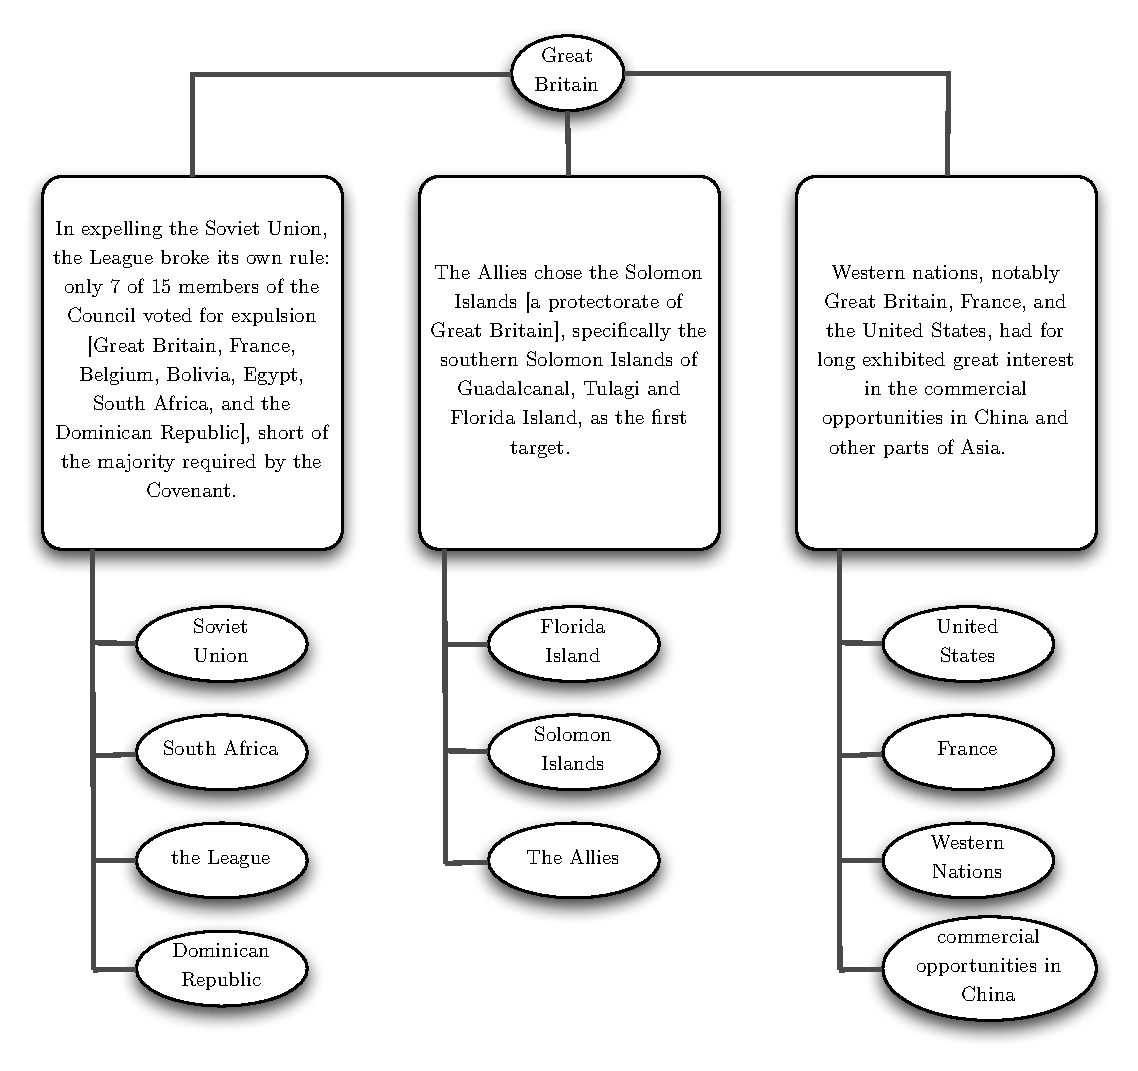
\includegraphics[width=\textwidth]{connection_diagram}
    \caption{Connections from ``Great Britain''}
    \label{fig:gb-connections}
\end{figure}

While the word ``Britain'' does appear in each of these sentences, not every connection in this graph relies on such a match.  For instance, ``Britain'' also has a vertex leaving it with the sentence ``As agreed with the Allies at the Tehran Conference (November 1943) and the Yalta Conference (February 1945), the Soviet Union entered World War II's Pacific Theater within three months of the end of the war in Europe.''  This link arises from a property found elsewhere which states that the entity ``Britain'' is a constituent part of the entity ``Allies'' which also maps to ``Western Allies'' among other forms.  This connection is a prime example of the potential power of this process.

One of the connections formed by the above vertex is to the entity ``the Molotov-Ribbentrop pact''---the non-aggression pact formed by the Soviet Union and Germany prior to World War II, later broken by Germany's invasion of the Soviet Union.  Another connection is formed to the entity ``Romania'' which is one of the countries Germany and the Soviet Union secretly agreed to divide in their pact.

The entity ``Britain'' is connected to the entity ``the Molotov-Ribbontrop pact'' via a sentence which contains neither phrase yet is a sound, historically-valid connection.  Germany's violation of the pact led to the Soviet Union's alliance with the Allied forces, of which Britain was a key member, for the duration of World War II and two key events brought about by this alliance were the Tehran and Yalta Conferences.  This connection makes perfect sense.

This example shows how my process can produce logical, sound connections without the string forming an entity being present in said connections.  While most connections are not as strong or interesting as this, examples like this one show the promise of my solution.

Indeed, most connections do appear to be based on string matches, though this is not the case.  This stems from the heavy use of the Stanford NLP library's coreference resolution, used to provide context to the ambiguous pronouns which often form an entity.  Doing so has the side effect of creating connections due to the presence of a string.  In effect, a connection which likely would have been found regardless is made stronger by the presence of such a token.

\section{False Positive Examples}

While this graph does contain many useful and interesting entities and connections, there are also many strange connections for which I have not been able to find explanations.  For instance, the following sentence produces a property about Britain which bears no basis in history: ``Upon leaving the meeting, Mussolini was arrested by `carabinieri' and spirited off to the island of Ponza.''  This sentence refers to the ousting of Mussolini immediately before Italy's surrender.  While Britain is of course connected to this event, the textual justification for this specific connection is incorrect.  

More evaluation is needed to determine the specific reasons for such false positives.  In small-scale testing, likely explanations fall broadly into two categories: incorrect coreference resolution by the Stanford library and poorly-formed properties.  The former problem cannot be easily solved but the latter is likely due to a set of properties which does not sufficiently encompass every needed possibility.  That is, a property is being defined which, while needed, is not specific enough and yields an ambiguous or strange result.  A better-defined set of properties is needed to alleviate this problem.


\chapter{Future Recommendations} 
\label{chp:recs}
During the course of my research I encountered several ideas which I eschewed for the sake of simplicity.  Having completed this thesis I realize now that this was a mistake and the ideas presented in this section would, I believe, produce a far stronger result than my current approach.

\section{Higher Order Dependency Relations}

In its current form, my algorithm only takes into account immediate dependency relationships.  Within the dependency tree of a sentence, only dependency relationships of nodes and their immediate descendants are directly used.  More research is needed to determine the usefulness of what I term ``higher-order dependency relations''---relationships which ``leap-frog'' a node and act on a governor and its dependent's dependents.

In figure~\ref{fig:dep-graph} this would manifest itself as a relationship between \verb|GAVE| and \verb|MY|.  The most obvious challenge concerns the exact type of the function used.  In this instance the relationship is a combination of direct object and possessive relationships.  Furthermore, this increases the space of possible functions from approximately fifty to 1225 assuming that the graph of possible combinations is complete.  Manually defining such a large number of functions is not feasible.  

While this approach could produce interesting results, it is likely not practical.

\section{Using the Simple English Wikipedia}

Ruiz-Casado et al \cite{Ruiz-casado05automaticassignment} used the Simple English edition of Wikipedia in their work.  Such an approach has several benefits: its simpler sentences would likely reduce problems in successfully parsing articles and its clearer grammar is less likely to rely on nuance to convey information.  In their research the Simple English edition was chosen for the same reasons.  Simpler syntactic structures are much easier to handle.

\section{Machine Learning}

Were I to redo my research I would begin by using a machine learning approach.  Rather than manually programming dependency functions I would annotate a large set of sentences with the properties conveyed by dependency functions or common compositions of functions.  Using machine learning these hand-annotated sentences would form the training corpus and would potentially produce a more encompassing set of functions.  

\section{A Probabilistic Approach}

Closely related to a machine learning approach, and indeed intertwined in many ways, would be the inclusion of probability.  Currently all properties produced are accepted at face value---their weight comes from the number of times that property or a similar property is produced.  While this allows for a rough approximation of probability, this could be extended.  For example, within dependency functions there is likely room to account for the likelihood of a property being true based on the probability of what nearby relations consist of.

\appendix

\chapter{Some Relevant NLP Concepts}

\section{Dependency Grammars}     

Dependency grammars are a class of grammatical theory not based on context-free grammars but instead on the relations between words.  (Jurafsky, 354).  This class of theory was first explored by early Greek and Indian linguists and regained popularity in the latter 20th century.  

Dependency grammars are quite simple: every word in a sentence is dependent upon another word (save for the head or root word) and these relationships form a tree structure as seen in the figure below.  Furthermore, each relationship has a type.  This structure abstracts word order away, meaning that multiple sentences can map to the same dependency tree.

Various specific grammars exist for the English language; the grammar used here is that employed by the Stanford library which defines 55 semantic relations.

\begin{figure}
\setlength{\unitlength}{0.8cm}
\begin{picture}(12,10)
	\put(1,9){$<ROOT>$}
	\put(2.8,8.8){\line(1,-2){0.6}}
	\put(3,7){$GAVE$}
	\put(2.5,5.6){\line(1,2){0.6}}
	\put(1.3,6.2){nsubj:}
	\put(2,5){$I$}
	\put(3.9,6.8){\line(1,-2){0.6}}
	\put(3.1,6.2){iobj:}
	\put(4,5){$HIM$}
	\put(4.8,7){\line(1,-1){1.4}}
	\put(5.8,6.2){dobj:}
	\put(6,5){$ADDRESS$}
	\put(5.5,3.5){\line(1,2){0.6}}
	\put(4.5,4){poss:}
	\put(5,3){$MY$}
\end{picture}
\caption{Dependency Graph for ``I gave him my address'' \cite{nlpbook}}
\label{fig:dep-graph}
\end{figure}

In this sample sentence, ``I gave him my address,'' we can see how $GAVE$ is the root word of this sentence, that is it has no governor word.  Every other word in the sentence is a dependent of another word and each of these dependencies has a type.  The relationship between $I$ and $GAVE$ is given as $nsubj(gave-2, I-1)$, indicating a \emph{nominal subject} relationship between the tokens ``gave'' and ``I'' at indices 2 and 1, respectively.

\section{Why dependency grammars?}

Dependency grammars appealed to me for a number of reasons: functionalism, the simplicity of representing a sentence as a tree and their potential for property extraction.  This form allows for verbs to be viewed as infix functions and identifies their arguments.  Doing so helps quickly extract statements of the type ``$Entity_{i}$ modifies $Entity_{i+1}$'' and bind both these entities and the type of modification to a given instance.  Doing so establishes relationships between entities and properties of those entities.  

Essentially, dependency grammars help reduce complex sentences to less-complex relations, greatly simplifying the task of extracting these relationships from a document.  While a tremendous amount of contextual information is lost, the tradeoff allows for a small set of relatively simple functions to extract information from a wide range of input documents.  




\chapter{Tools Used}

This appendix briefly enumerates the tools, languages and libraries used to complete this thesis.

\begin{description}
\item[Scala] The primary implementation language, described in section~\ref{sec:why-scala}.
\item[Java] Glue code for interfacing with the Stanford NLP Library was written in Java.
\item[SBT] The Simple Build Tool, part of the Scala ecosystem, was used as the build and dependency manager.
\item[Play! Framework] A web framework written in Scala, used for constructing a visual front-end.
\item[Stanford NLP Library] Described extensively in section~\ref{sec:stanford-lib}.
\item[PostgreSQL] Originally stored graph data in a PostgreSQl database but later transistioned to MySQL.
\item[MySQL] Used to store graph data for both its easier to use fulltext searches and availability on department machines.
\item[Squeryl] A Scala library for interfacing with databases.
\item[Bliki] A wiki-markup library used to strip Wikipedia articles of their markup.
\end{description}

% \chapter{Code Highlights}


\nocite{nlpdeps,nlpfparse,nlpparser}


% FIX THIS -- refs.bib is the bibtex file
\bibliography{refs}
\bibliographystyle{IEEEtran}


\end{document}
